% figure: 频域-相角合成三角形.png
% 用途：自控 05-1-1 例1 ⑤ —— 相角合成的辅助直角三角形
%       tan α = ωT，cos α = 1/√(1+ω²T²)，斜边 √(1+ω²T²)。
% 构建：..\build.ps1 -File .\geom-alpha-triangle.tex
% 说明：夹角由两直角边 7 : 3.5 定死 = 26.57°；角弧终点与斜边标签的 rotate
%       都用这个数，改边长时必须同步改（atan(3.5/7) = 26.57°）。
\documentclass[border=8pt]{standalone}
\usepackage{fontspec}
\setmainfont{Cambria}
\usepackage{unicode-math}
\setmathfont{Cambria Math}
\usepackage{tikz}
\usetikzlibrary{calc}
\usepackage{xcolor}

\definecolor{figink}{HTML}{1E2228}      % 图线主色
\definecolor{figacc}{HTML}{B23020}      % 强调色（角弧/角名）
\definecolor{figfill}{HTML}{E8EFF8}     % 三角形填充
\definecolor{figsub}{HTML}{606874}      % 次要文字与参考轴

\begin{document}
\begin{tikzpicture}[x=1cm, y=1cm, line width=1.1pt, line cap=round, line join=round]
  \coordinate (O) at (0,0);
  \coordinate (A) at (7,0);
  \coordinate (B) at (7,3.5);

  % 参考轴：贴着三角形外侧，不和直角边重合
  \draw[figsub, line width=0.4pt] (-0.5,-0.5) -- (7.2,-0.5);
  \draw[figsub, line width=0.4pt] (-0.5,-0.5) -- (-0.5,4.1);

  % 三角形本体
  \fill[figfill] (O) -- (A) -- (B) -- cycle;
  \draw[figink, line width=1.6pt] (O) -- (A) -- (B) -- cycle;

  % 直角标记
  \draw[figink, line width=1.0pt] ($(A)+(-0.45,0)$) -- ($(A)+(-0.45,0.45)$) -- ($(A)+(0,0.45)$);

  % 角弧（半径 1.5，落在夹角内）
  \draw[figacc, line width=1.0pt] (O) ++(1.5,0) arc (0:26.57:1.5);

  % 标签
  \node[figacc] at (2.25,0.55) {$\alpha$};
  \node[figink] at (3.5,-0.52) {$1$};
  \node[figink] at (7.75,1.75) {$\omega T$};
  \node[figink, rotate=26.57] at (3.2,1.85) {$\sqrt{1+\omega^{2}T^{2}}$};

  % 图例（横排两行，避免图面过高）
  \node[figink, anchor=west] at (0,-1.35) {$\tan\alpha=\omega T$};
  \node[figsub, anchor=west] at (0,-2.05) {$\cos\alpha=\dfrac{1}{\sqrt{1+\omega^{2}T^{2}}}$};
\end{tikzpicture}
\end{document}
